 %Tipo de documento
\documentclass[12pt,a4paper]{article}

%Idioma y caracteres del idioma
\usepackage[utf8]{inputenc}
\usepackage[spanish]{babel}
\usepackage{natbib}
\usepackage{multirow}
\usepackage[table,xcdraw]{xcolor}
%Opción para incluir gráficos
\usepackage{graphicx}

%Opciones para incluir caracteres matemáticos
\usepackage{amsmath}
\usepackage{amsfonts}
\usepackage{amssymb}
\usepackage{url}

%Opciones de márgenes
\usepackage[left=3cm,right=3cm,top=2.5cm,bottom=2.5cm]{geometry}

%Opciones para poner dos subfiguras
\usepackage{subcaption} 

\begin{document}

%Todo esto es la portada - >

\begin{titlepage}

\begin{center}
\begin{figure}[htb]
\begin{center}

\includegraphics[scale=0.7]{Figuras/logounab.png}
\end{center}
\end{figure}

\vspace*{2cm}

UNIVERSIDAD ANDRÉS BELLO

FACULTAD DE INGENIERÍA

INGENIERÍA CIVIL INDUSTRIAL

\vspace*{3cm}

\begin{Large}
\textbf{Modelo de asignación de vehículos de recolección de escombros en desastres naturales}
\end{Large}

\vspace*{3cm}

Isaac Eliseo Montero Jara

\vspace*{0.5cm}

Samantha Camila Reid Calderón

\vspace*{2.5cm}

\begin{flushright}

TRABAJO DE TESIS PRESENTADO EN CONFORMIDAD 

A LOS REQUISITOS PARA OBTENER EL GRADO DE 

INGENIERO CIVIL INDUSTRIAL

\end{flushright}

\vspace{2cm}

SANTIAGO - CHILE

2020

\end{center}

\end{titlepage} % <- Hasta acá termina la portada

%Pagina de declaración que hiciste las cosas tú

\pagebreak

\begin{center}
\begin{figure}[htb]
\begin{center}

\includegraphics[scale=0.7]{Figuras/logounab.png}
\end{center}
\end{figure}

\vspace*{2cm}

FACULTAD DE INGENIERÍA \vspace*{0.5cm}

INGENIERÍA CIVIL INDUSTRIAL \vspace*{0.5cm}

DECLARACIÓN DE ORIGINALIDAD Y PROPIEDAD

\end{center}

\vspace*{3cm}

Yo, Isaac Eliseo Montero Jara, declaro que este documento no incorpora material de otros autores sin identificar debidamente la fuente. 

\vspace*{4cm}

\begin{flushright}
Santiago, XX del 2020

\vspace{3.5cm}

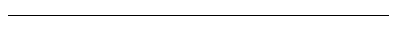
\includegraphics[scale=0.7]{Figuras/linea.png}

Firma del alumno

\end{flushright}

\pagebreak		% <----- Término de declaración


%Aquí se pone una frase inspiradora

\vspace*{20cm}

\begin{flushright}

\textit{"La educación es la llave para abrir el mundo, un pasaporte a la libertad.\\ Oprah Winfrey"}

\end{flushright}

\pagebreak % <--------- Término de frase inspiradora

% Agradecimientos a la vida


\begin{large}

\textbf{Agradecimientos}

\end{large}

\vspace*{1cm}

En primero lugar agradezco a mi padre Hernán Montero Gonzalez, que me ha brindado las herramientas y amor necesario para poder lograr mis objetivos propuestos en la vida. 

Agradezco a mi Madre Jacqueline Jara Peréz, sólo el hecho de creer en mí durante mi niñez y darme a entender que puedo ser capaz de todo lo que me proponga.

Agradezco a mi novia Valentina Calderón, la cual me brindó la energía y apoyo incondicional para lograr mis objetivos profesionales. 

Agradezco a mis familiares, los cuales me ayudaron en etapas donde más lo necesitaba. 

Agradezco a mi profesor de tesis Samantha Reid, y también a Franco Menares, los cuales fueron un apoyo fundamental para lograr esta investigación.

\pagebreak			% <-------- Fin te página de agradecimientos

\tableofcontents	% <--------- Se genera la tabla de contenidos, solita!!!

\pagebreak

\listoftables		 % <--------- Se genera la tabla de tablas, solita!!!

\listoffigures		% <--------- Se genera la tabla de figuras, solita!!!

\pagebreak

\section{CONTEXTO}

\subsection{INTRODUCCIÓN}

Históricamente se han registrado numerosos eventos, denominados desastres. \citet{van2006humanitarian} los define como interrupciones que afectan físicamente a un sistema en su conjunto y amenaza sus prioridades y objetivos. Existen dos tipos de desastres: los provocados por el hombre (tecnológicos, ataques terroristas, ente otros); y los ocasionados de forma natural. Estos últimos se clasifican en: meteorológicos (tornados, huracanes, incendios); hidrográficos (inundaciones, tormentas, tsunamis); y geofísicos (volcánicos y terremotos).

Según EM-DAT (2019), en la última década, a nivel global, se realizó un registro de 3155 desastres naturales, produciendo más de 430.000 fallecidos, 1.300 millones de personas afectadas, y daños aproximados 1.340 billones de dólares.

\subsection{LOGÍSTICA HUMANITARIA}
La logística humanitaria se define como el proceso de planificación, implementación y control, del flujo eficiente, rentable y almacenamiento de bienes y materiales, así como la información relacionada, desde el punto de origen hasta el punto de consumo con el fin de aliviar el sufrimiento de las personas vulnerables \citep{supply}. Por otra parte, \citet{celik} establece que, si bien la logística humanitaria desempeña un papel importante en la consecución de los objetivos de la ayuda humanitaria, existen grandes diferencias y desafíos en comparación con la logística en las aplicaciones comerciales. En resumen, la logística humanitaria se centra en brindar atención a personas frente a un desastre natural.

Según \citet{celik}, la gestión de desastres se puede dividir en cuatro fases, cada una correspondiente al ciclo de vida de un desastre: mitigación, preparación, respuesta, recuperación. En las dos primeras fases se ven los temas orientados a gestionar antes de un desastre; en respuesta se ven las primeras 72 horas después de un desastre; y en recuperación las actividades orientadas después de hacer trascurrido estas 72 horas. El objetivo principal en recuperación es restaurar y estabilizar el sistema en la sociedad y las actividades realizadas son: eliminación y reciclaje de desechos tanto como de la población como del desastre, restauración de la red e infraestructura y la distribución de productos básicos de socorro.

\subsection{FASE DE RECUPERACIÓN}

La recuperación comienza cuando la emergencia se ha estabilizado, por lo que ya no existe una amenaza latente a la población, y termina cuando la comunidad se ha recuperado. El objetivo de la mayoría de las personas es reanudar sus vidas exactamente antes de que ocurriera el desastre, tanto en el ámbito material como psicológico. Además las entidades deben reparar los daños correspondientes a sus instalaciones físicas, tanto comerciales, publicas e industriales\citep{lindell2006wiley}.

Según \citet{Feng2003} existen dos tipos de actividades en la fase de recuperación. Las primeras comienzan posterior a un desastre y en un trascurso de 72 horas posteriores y se centran en despejar las vías de locomoción para agilizar el traslado de la población afectada, disminuyendo el daño a la sociedad. Posteriormente, se realizan actividades a largo plazo, cuyo objetivo es eliminar el rastro físico que dejo el evento, enfocándose en reciclar, trasladar, almacenar, reducir los desechos, mencionando que estas actividades pueden tardar meses o años.

\subsection{CONTEXTO NACIONAL}

Según \citep{emdat}, durante la última década en Chile, se registraron 21 eventos. Estos han provocado 815 pérdidas humanas y más de 10.000 lesionados, además de afectar a 4.100.000 personas en su vida cotidiana y dejando a 834.500 personas sin hogar. Además, en lo económico, se han generado daños cercanos a los 34.200 millones de dólares. En la figura \ref{fig:figura1} se visualiza el total de personas por tipo de desastre, predominando el tipo geofísico.

\begin{figure}[h!]
\centering
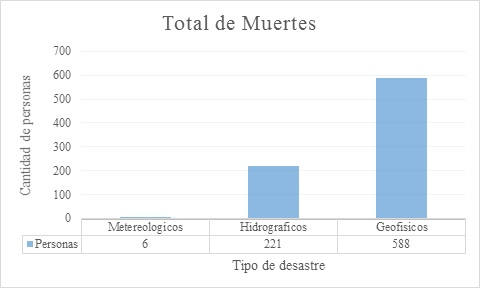
\includegraphics[scale=0.8]{Figuras/g1.jpg}
\caption{Totalidad de personas muertas por desastres naturales última década. Fuente: EM-DAT (2019)}
\label{fig:figura1} 
\end{figure}

\section{IMPORTANCIA DEL TRABAJO}

La importancia de este trabajo radica en un bienestar social para la población afectada posterior a un desastre, además de prestar apoyo a las actividades logísticas involucradas dentro de un desastre. Prestando el enfoque al tipo de desastre con mayor número de muertes 588 en la última década, este estudio se va a centrar en el tipo de desastre geofísico, además de presentar daños en infraestructura en cifras de billones de dolares \citep{emdat}. La recolección de escombros en las primeras 72 horas de operación debe estar destinada a los edificios más importantes dentro de la logística humanitaria, considerando que es vital tener las vías de acceso  tales como hospitales, colegios y albergues. Estos edificios impactan directamente a la ayuda de las personas afectadas, brindando atención de urgencia a los heridos y proporcionando albergues a las víctimas cuyos hogares han quedado inhabilitados. Asimismo, prestando importancia, al termino volver a la normalidad, favoreciendo a la población, a volver a sus actividades diarias, y restaurar la salud psicológica de la población \citep{celik}. 

%%%%%%%%%%%%%%%%%%%%%%%%%%%%%%%%%%%%%%%%%%%%%%%%%%%%%%%%%%%%

%Aquí rellenar o ordenar más según lo que tienes en la PPT. Es decir, poner que las mayores causas son por: 1) los desastres provocan muchos muertes y perdida monetaria; 2) La recolección de escombros permiten tener acceso a hospitales, albergues y carreteras; 3) Restaura física y psicologicamente a la población. Cada uno de esos tres ítemes los mencionas, los describes brevemente y le pones la REF a cada una.

%%%%%%%%%%%%%%%%%%%%%%%%%%%%%%%%%%%%%%%%%%%%%%%%%%%%%%%%%%%%

\section{DISCUSIÓN BIBLIOGRÁFICA}

Tras ocurrido un desastre, es importante recuperar la vida previa a la comunidad. Uno de los elementos a considerar son las políticas de reconstrucción y restauración de las redes \citet{Feng2003}. Por lo mismo, se deben encontrar soluciones que permitan optimizar el uso de los recursos destinados a actividades de limpieza y recolección.

\subsection{RUTEO VEHICULAR}

Existen distintos autores que abordan el problema a través de ruteo vehicular. \citet{Karlaftis2007} proponen un modelo de tres etapas, donde maximiza la importancia de los nodos, asigna recursos y minimiza costos de reparación, enfocado en puentes. \citet{Liberatore2014} minimizan el tiempo necesario para las reparaciones de emergencia y distribución de artículos de ayuda a través de un modelo multicriterio, donde incorpora el tiempo, costo, confiabilidad, seguridad y satisfacción de la demanda. \citet{Aksu2014} maximiza la accesibilidad a la red para evacuar a los sobrevivientes y remover desechos de las rutas. \citet{MayaDuque2016} realizan una planificación de equipos de limpieza y su ruteo dentro de la red para limpiar edificios. Por último, \citet{Kasaei2016} desarrollan un modelo lineal que limpia caminos bloqueados, minimizando el tiempo de reconexión de la red y maximizando el beneficio total de reconexión dentro de un tiempo dado.

\subsection{PLANIFICACIÓN Y ASIGNACIÓN}

De manera similar, existen estudios que abordan el problema a través de planificación y asignación. \citet{Feng2003} proponen un modelo multiobjetivo de limpieza de edificios, donde maximiza el largo de las rutas accesibles, el total de vidas salvadas y minimiza el riesgo. \citet{Brooks2013} determinan la estrategia para asignar los vehículos entre los sitios de recogida y almacenamiento temporal de escombros, maximizando el flujo de la red. \citet{Ransikarbum2016} desarrollan un modelo para decisiones estratégicas en la distribución de suministros y restauración de la red, maximizando equidad, minimizando demanda insatisfecha y costos. \citet{Akbari2017} generan una planificación para equipos de limpieza para reconectar la red.

\subsection{RECICLAJE}

Además, en los últimos años se ha incorporado el factor de reciclaje en esta fase. \citet{Boonmee2018} realizan un modelo de localización y asignación de centros de reciclaje, minimizado los costos y penalizando daños al ambiente. \citet{Wang2019} proponen un modelo de asignación multiobjetivo que minimiza costos de remoción de escombros, tiempo total de procesamiento y maximiza el reciclaje.

En la tabla \ref{tab:tabla1} se resume toda la información de la revisión de la literatura, junto con las leyendas abajo.

\begin{table}[h!]
\resizebox{16cm}{!} {
\begin{tabular}{l|c|l|c|c|c|c|c|c|c}
\hline
Autor & Año & Objetivo(s) & Tipo & Decisión & Limpieza & 1 & 2 & 3 & 4 \\ \hline

\multirow{3}{*}{\citeauthor{Feng2003}} & \multirow{3}{*}{\citeyear{Feng2003}} & Maximizar largo de las rutas accesibles & \multirow{3}{*}{M} & \multirow{3}{*}{A} & \multirow{3}{*}{E} & \multirow{3}{*}{}  & \multirow{3}{*}{x}  & \multirow{3}{*}{ } & \multirow{3}{*}{ } \\ \cline{3-3}
& & Maximizar total de vidas salvadas &  &  &  & & & & \\ \cline{3-3}
& & Minimizar riesgo &  &  &  & & & & \\ \hline

 
\multirow{3}{*}{\citeauthor{Karlaftis2007}} & \multirow{3}{*}{\citeyear{Karlaftis2007}}                      & Maximizar importancia de los nodos & \multirow{3}{*}{M} & \multirow{3}{*}{R} & \multirow{3}{*}{E}  & \multirow{3}{*}{}  & \multirow{3}{*}{ } & \multirow{3}{*}{}  & \multirow{3}{*}{} \\ \cline{3-3}
& & Maximizar  asignación de recursos &  &  &  & & & & \\ \cline{3-3}
& & Minimizar costos de reparación &  &  &  & & & & \\ \hline
 

\citeauthor{Brooks2013} & \citeyear{Brooks2013} & Maximizar flujo en la red                           & S & A & C & & x & x & \\ \hline

\multirow{2}{*}{\citeauthor{Aksu2014}} & \multirow{2}{*}{\citeyear{Aksu2014}} & Maximizar accesibilidad en la red para evacuación & \multirow{2}{*}{S} & \multirow{2}{*}{R} & \multirow{2}{*}{C}  & \multirow{2}{*}{}  & \multirow{2}{*}{x}  & \multirow{2}{*}{} & \multirow{2}{*}{} \\
 & & para sobrevivientes y remover los desechos de las rutas &  &  &  & & & & \\ \hline

\multirow{2}{*}{\citeauthor{Liberatore2014}} & \multirow{2}{*}{\citeyear{Liberatore2014}}                      & Minimizar tiempo de reparaciones & \multirow{2}{*}{S} & \multirow{2}{*}{R} & \multirow{2}{*}{C}  & \multirow{2}{*}{}  & \multirow{2}{*}{x}  & \multirow{2}{*}{ } & \multirow{2}{*}{} \\
& & de emergencia y distribución &  &  &  & & & & \\ \hline    
    
    
\multirow{2}{*}{\citeauthor{Kasaei2016}} & \multirow{2}{*}{\citeyear{Kasaei2016}}                      & Maximizar tiempo de reconexión de la red & \multirow{2}{*}{M} & \multirow{2}{*}{R}  & \multirow{2}{*}{C} & \multirow{2}{*}{}  & \multirow{2}{*}{} & \multirow{2}{*}{} & \multirow{2}{*}{x} \\ \cline{3-3}
& & Maximizar beneficio al reconectar la red & & & & & & & \\ \hline
     
                
\citeauthor{MayaDuque2016} & \citeyear{MayaDuque2016} & Maximizar cantidad de edificios limpiados & S & R & E & & x & & \\ \hline


\multirow{2}{*}{\citeauthor{Ransikarbum2016}} & \multirow{2}{*}{\citeyear{Ransikarbum2016}}                      & Maximizar equidad & \multirow{2}{*}{M} & \multirow{2}{*}{A}  & \multirow{2}{*}{C} & \multirow{2}{*}{}  & \multirow{2}{*}{}  & \multirow{2}{*}{} & \multirow{2}{*}{x} \\ \cline{3-3}
& & Minimizar demanda insatisfecha & & & & & & & \\ \hline


\citeauthor{Akbari2017} & \citeyear{Akbari2017} & Maximizar cantidad de edificios limpiados                               & S & A & C & & x & x & \\ \hline


\citeauthor{Boonmee2018} & \citeyear{Boonmee2018} & Minimizar costos, penalizando daño al medio ambiente & S & A & E & x & & & \\ \hline


\multirow{3}{*}{\citeauthor{Wang2019}} & \multirow{3}{*}{\citeyear{Wang2019}}                      & Minimizar los costos de remoción de escombros & \multirow{3}{*}{M} & \multirow{3}{*}{A} & \multirow{3}{*}{E}  & \multirow{3}{*}{x} & \multirow{3}{*}{}  & \multirow{3}{*}{}  & \multirow{3}{*}{} \\ \cline{3-3}
& & Minimizar tiempo total & & & & & & & \\ \cline{3-3}
& & Maximizar reciclaje & & & & & & & \\ \hline


\multirow{2}{*}{Propuesta} & \multirow{2}{*}{2020} & Maximizar preferencia de limpieza en la red                        & \multirow{2}{*}{S} & \multirow{2}{*}{A} & \multirow{2}{*}{E} & \multirow{2}{*}{} & \multirow{2}{*}{x}  & \multirow{2}{*}{} & \multirow{2}{*}{} \\
& & en los primeros días de trabajo & & & & & & & \\ \hline
\end{tabular}
}

\resizebox{8cm}{!} {
\begin{tabular}{ l l }
\\
Tipo: 	& S - Modelo monobjetivo; M - Modelo multiobjetivo \\
Decisión: & R - Ruteo vehicular; A - Asignación y planificación \\
Limpieza: & E - Edificios; C - Caminos \\
(1)		& Reciclaje \\
(2)		& Tiempo \\
(3)		& Almacenamiento Temporal \\
(4)		& Distribución de suministros 
\end{tabular}
}
\caption{Revisión de la literatura; Fuente: Elaboración propia}
\label{tab:tabla1}
\end{table}

%%%%%%%%%%%%%%%%%%%%%%%%%%%%%%%%%%%%%%%%%%%%%%%%%%%%%%%%%%%%

% Intentar sacarle los espacios entre objetivos. Sino, no importa

%%%%%%%%%%%%%%%%%%%%%%%%%%%%%%%%%%%%%%%%%%%%%%%%%%%%%%%%%%%%

\section{CONTRIBUCIÓN DEL TRABAJO}

La contribución de este trabajo radica en: (a) agregar un ponderador de preferencia de limpieza y por día a los edificios, el cual beneficia la recolección en los primeros días; (b) el caso de estudio se efectúa con datos reales de la región de Iquique, en conjunto con datos de simulación del programa HAZUS. 

\section{HIPÓTESIS}

Al incorporar un factor de preferencia por día y edificio, se puede planificar de mejor manera la recolección en un horizonte de tiempo.

\section{OBJETIVO GENERAL}

Desarrollar una metodología que permita determinar la asignación de vehículos de recolección dentro de un horizonte de planificación, en la fase de recuperación temprana de un desastres natural.

\section{OBJETIVOS ESPECÍFICOS}

\begin{itemize}
	\item Desarrollar modelo de optimización para el problema.
	\item Obtener y depurar datos de Iquique.
	\item Obtener datos con software HAZUS.
	\item Obtener resultados y aplicar análisis de sensibilidad.
\end{itemize}

\section{Caso de Estudio}

\subsection{Área de estudio}

El caso de estudio se realizó en la región de Tarapacá en la ciudad de Iquique, Chile, visualizada en la \ref{fig:fig2}. Esta ciudad cuenta con una población de 191.468 personas y una superficie de 2.262,4 $m^{2}$ \citep{CENSO2017}.

\begin{figure}[h!]
\centering
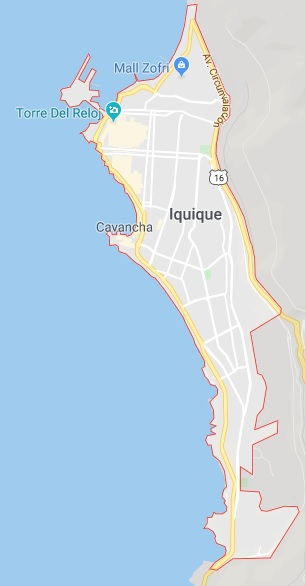
\includegraphics[scale=0.65]{Figuras/iquique1.jpg}
\caption{Mapa de Iquique. Fuente: Google Maps (2019)}
\label{fig:fig2}
\end{figure}

Esta región está propensa a sufrir catástrofes naturales debido a su ubicación sobre la placa Sudamericana la cual produce un movimiento contrario a la placa de Nazca \citep{sismologia}. Según \citet{emdat}, se cuenta con un historial de cuatro sismos de gran magnitud en los últimos 25 años, debido a que superan los 7.0 grados de magnitud. En la Tabla \ref{tab:tab1} se muestran los eventos sísmicos desde 1900, cuyas leyendas son: Magnitud de ondas superficiales (Ms) y Magnitud del momento (Mw) \citep{sismologia}.

\begin{table}[h!]
	\centering
	\begin{tabular}{c|c|c|c|c} \hline
	Fecha	& Latitud &	Longitud & Magnitud  Ms / Mw & Profundidad (km) \\ \hline
	15-09-1911  & -20	& -72 	 & 7.3 (Ms) & - \\ 
	23-02-1933  & -20   & -71	 & 7.6 (Ms) & 40  \\ 
	01-12-1943  & -21	& -69    & 7   (Ms) & 100 \\ 
	25-04-1949	& -19.75& -69	 & 7.3 (Ms) & 110 \\ 
	08-01-1956	& -19   & -70	 & 7.1 (Ms) & 11 \\ 
	13-06-1959	& -20.42& -69 	 & 7.5 (Ms) & 83 \\ 
	29-11-1976 	& -20.52& -68.919& 7.3 (Ms) & 82  \\ 
	08-08-1987	& -19	& -70	 & 7.1 (Ms) & 42  \\ 
	13-06-2005	& -19.895&-69.125& 7.8 (Ms/Mw) & 108 \\ 
	01-04-2014	& -19.572&-70.908& 8.2 (Mw) & 38.9  \\ \hline
	\end{tabular}
	\\
	\caption{Historial de terremotos Región de Tarapacá, a partir del año 1900. Fuente: \citep{guc}}.
	\label{tab:tab1} 
\end{table}

\subsection{Recopilación de datos}

\subsubsection{Red vial y obtención de escombros}

La red vial se obtuvo a través del Ministerio de Transporte y Telecomunicaciones de Chile, la cual se compone de 1655 manzanas censales \citet{CENSO2017}. Estos datos fueron procesados en el software ArcGis 10.1, del cual se obtuvo la matriz de distancia entre los nodos de la red.

Por otro lado, la cantidad de escombros para cada una fue obtenida a través del software HAZUS 2.1, a partir de una simulación de un escenario de magnitud 8.0 Mw. Se tomó en consideración sólo los escombros de tipo madera y ladrillos, puesto que los demás requieren de equipamiento más avanzado \citep{hasuz}.

\subsubsection{Edificios}

Durante la fase de recuperación es importante mantener las vías de acceso despejadas a hospitales, colegios y otros edificios de interés. Estos se utilizan como recurso para la comunidad con el fin de albergar personas y/o prestar servicios de primeros auxilios \citet{lindell2006wiley}. En total, se consideraron 16 centros de salud y 65 establecimientos de educación, cuyo detalle se presenta en el Anexo \ref{anexo1} y su distribución espacial en la Figura \ref{fig:fig3}.

\begin{figure}[h!]
	\centering
	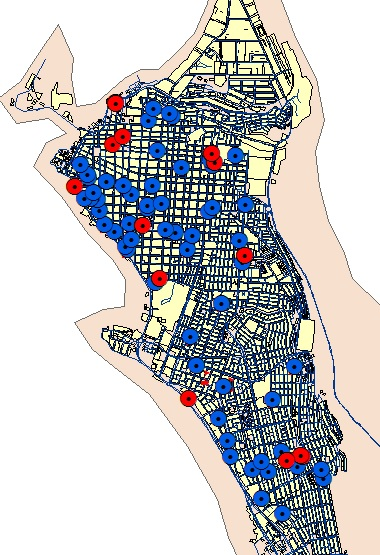
\includegraphics[scale=0.65]{Figuras/mapaarc.JPG}
	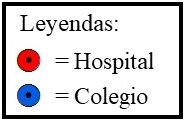
\includegraphics[scale=0.5]{Figuras/simb1.jpg}
	\caption{Centros de Salud y Establecimientos de Educación en Iquique. Fuente: Elaboración Propia en base a datos del CENSO (2017)}
	\label{fig:fig3}
\end{figure}

\subsubsection{Equipamiento vehicular}

Durante las labores de recolección de escombros se necesitan equipos de limpieza, los cuales deben tener las capacitaciones necesarias para poder utilizar maquinaria pesada tal como bulldozers, vehículos livianos y camiones recolectores \citep{Kasaei2016}.

El vehículo seleccionado es un camión IVECO modelo CAMIÓN TOLVA AD410 de potencia 420 HP y tracción 8x4. Se considera este camión transportador de escombros, el cual tiene una capacidad de transporte de 20 $m^3$ por viaje. Además, se considera una velocidad estándar de limpieza de $250 [m^{3}/h]$ \citep{Feng2003} y una velocidad de desplazamiento de $20000 [m/h]$. Finalmente, los vehículos cuentan con una capacidad de $4 m^{3}$ aproximadamente \citep{CAT}.

\subsubsection{Software}

Los modelos de optimización y simulación fueron ejecutados en AMPL Gurobi 8.1.0 y HAZUS 2.1, respectivamente. Además las instancias fueron desarrolladas por un computador con procesador Intel(R) Core (TM) i7-6700HQ @ 2.60 Hz (8 CPUs), con 12 GB en memoria RAM.

\section{RESULTADOS}

\subsection{Confección de los escenarios}

\subsubsection{Extracto de la zona}

Debido a que la metodología es un modelo matemático NP-Hard, se trabajó con un extracto de la zona de estudio, la cual corresponde a la zona norte de la ciudad. Se elige esta área debido a la  existencia de los edificios con mayor prioridad de ser limpiados en los primeros días de trabajo, como Hospitales y colegios, siendo estos considerados con un factor de preferencia de limpieza en el modelamiento propuesto.
La visualización del extracto se muestra en la Figura \ref{fig:fig4} y el detalle de la zona, junto con la cantidad de escombros por manzana censal, está en la Figura \ref{fig:fig5}. El área está conformada por 109 manzanas, 2 centros de salud, 5 establecimientos educacionales y un depósito.

\begin{figure}[h!]
	\centering
	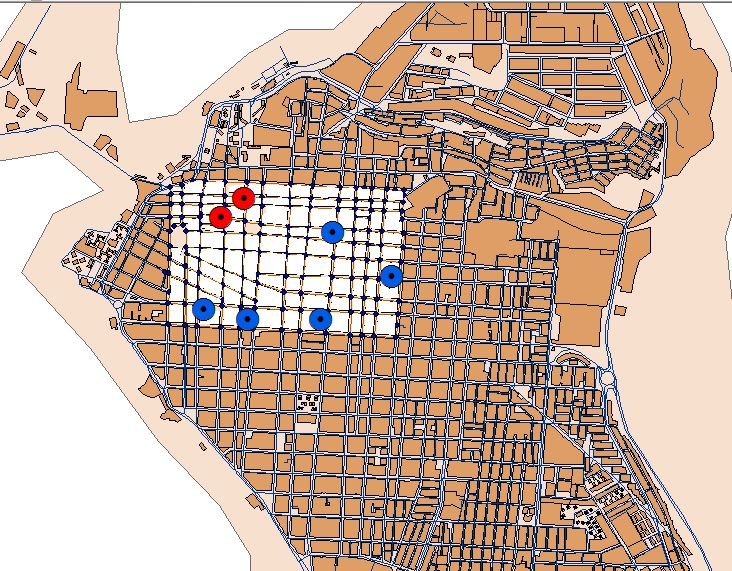
\includegraphics[scale=0.5]{Figuras/mapa2.jpg} 
	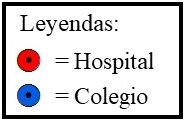
\includegraphics[scale=0.5]{Figuras/simb1.jpg}
	\caption{Extracto de la zona. Fuente: Elaboración propia.}
	\label{fig:fig4}
\end{figure}

\begin{figure}[h!]
	\centering
	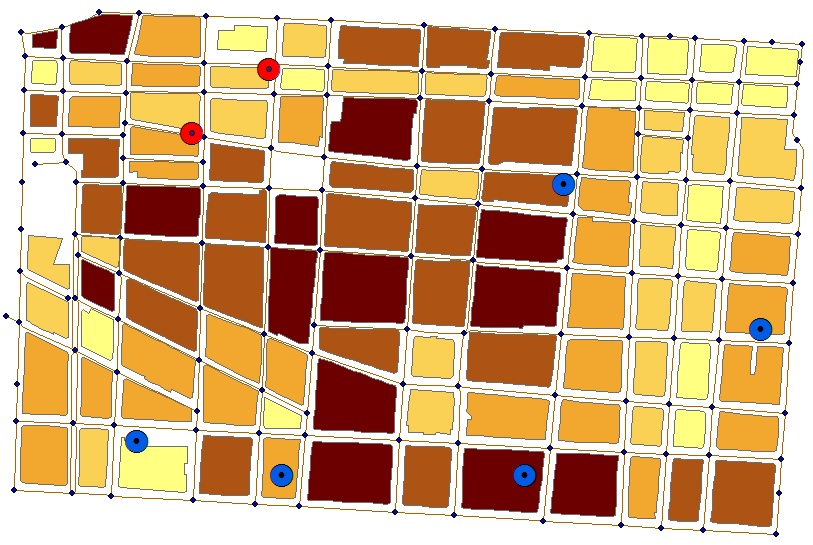
\includegraphics[scale=0.5]{Figuras/mapa1.jpg}
	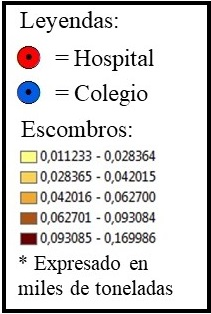
\includegraphics[scale=0.5]{Figuras/simb3.jpg} 
	\caption{Detalle del extracto de la zona con cantidad de escombros. Fuente: Elaboración propia.}
	\label{fig:fig5}
\end{figure}

\pagebreak

\subsubsection{Escenarios propuestos}

La ejecución del modelo se proponen siete escenarios, los cuales se detallan a continuación:

\begin{itemize}
	\item Escenario 0: Escenario Base.
	\item Escenario 1: Sin considerar el ponderador de prioridad.
	\item Escenario 2: 5 camiones operativos.
	\item Escenario 3: 15 camiones operativos.
	\item Escenario 4: Aumento del 10 \% volumen de escombros.
	\item Escenario 5: Aumento del 20 \% volumen de escombros.
	\item Escenario 6: Aumento del 30 \% volumen de escombros.
\end{itemize}

El Escenario 0 se analiza la situación actual, considerando una flota homogénea de 10 vehículos, 7 vueltas y un horizonte de planificación de 5 días. En el escenario 1 se analizan los resultados sin el factor de prioridad, para comparar su impacto. En los escenarios 2 y 3 se disminuye y aumenta el nivel en la flota, respectivamente. Por último, en los escenarios 4, 5 y 6 se analiza la variación aumentando los niveles en los volúmenes de escombros en 10\%, 20\% y 30\%, respectivamente.

\section{Análisis de la situación inicial (Escenario 0)}

En la situación actual, al considerar un terremoto de 8.0 Mw de magnitud, se obtienen los resultados de la Tabla \ref{tab:tab2}

\begin{table}[h!]
\resizebox{15cm}{!} {
\begin{tabular}{c|c|c|c|c|c|c|c|c|c}
\hline
\multirow{3}{*}{Escenario} & Función                   & Tiempo & GAP                   & Edificios                & Cant. prom. de                 & No. prom. de días & \multicolumn{3}{c|}{Cant. de días promedio de limpieza}                          \\ \cline{8-10} 
                           & \multirow{2}{*}{objetivo} & CPU    & \multirow{2}{*}{(\%)} & \multirow{2}{*}{Limpios} & escombros recolectados         & para limpiar      & \multirow{2}{*}{Hospitales} & \multirow{2}{*}{Colegios} & \multirow{2}{*}{Otros} \\
                           &                           & (seg)  &                       &                          & por día $M^{3}$ & un edificio       &                             &                           &                        \\ \hline
0                          & 103                       & 18000  & 1.33                  & 108                      & 1,254.97                         & 2.26              & 1                           & 1                         & 1.67                   \\ \hline
\end{tabular}
}
\caption{Detalle de modelamiento Escenario 0, Fuente: Elaboración propia.}
\label{tab:tab2}
\end{table}

%%%%%%%%%%%%%%%%%%%%%%%%%%%%%%%%%%%%%%%%%%%%%%%%%%%%%%%%%%%%%%%%%%%%%%%%%%%

%Arreglar la tabla para que quepa aquí, y poner los títulos correspondientes con letras

%%%%%%%%%%%%%%%%%%%%%%%%%%%%%%%%%%%%%%%%%%%%%%%%%%%%%%%%%%%%%%%%%%%%%%%%%%%%%

El modelo matemático se ejecutó por 5 horas, obteniendo un GAP del $1.33\%$. En esta instancia, se limpiaron 108 edificios, la cantidad de escombros recolectada es 3.761,23 $m^{3}$ .
En la Figura \ref{fig:esc0-graf} se presenta el gráfico de la cantidad de edificios limpiados por día, donde se aprecia que, a medida que pasan los días, se limpia una menor cantidad de edificios. Esto se justifica debido a que se le da prioridad al primer día de limpiar la mayor cantidad de nodos. Además se puede destacar que el modelo propuesto sólo utilizó 3 días de los 5 propuestos en el horizonte de planificación.


%%%%%%%%%%%%%%%%%%%%%%%%%%%%%%%%%%%%%%%%%%%%%%%%%%%%%%%%%%%%%%%%%%%%%%%%%%%

\begin{figure}[h!]
\centering
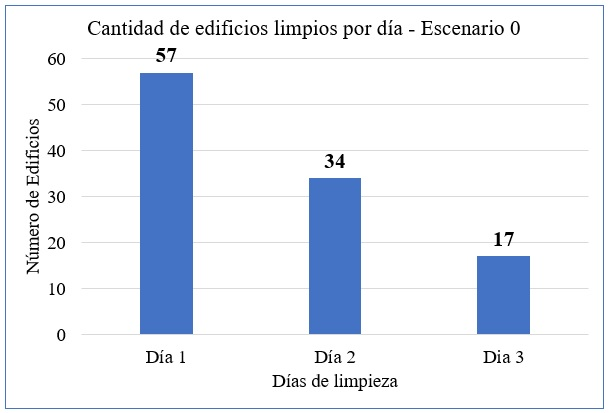
\includegraphics[scale=0.8]{Figuras/INDIC1.jpg} 
\caption{Detalle de edificios limpios (Escenario 0), Fuente: Elaboración propia}
\label{fig:esc0-graf}
\end{figure}

%%%%%%%%%%%%%%%%%%%%%%%%%%%%%%%%%%%%%%%%%%%%%%%%%%%%%%%%%%%%%%%%%%%%%%%%%%%%%

La distribución espacial de limpieza de los edificios se ve representada en la Figura \ref{fig:esc0-visu}, donde se visualiza cómo se van limpiando los edificios a medida que pasan los días. Aquí se observa la representación del factor de preferencia, limpiando una mayor cantidad de edificios el día 1 que al término de los días de limpieza.


%%%%%%%%%%%%%%%%%%%%%%%%%%%%%%%%%%%%%%%%%%%%%%%%%%%%%%%%%%%%%%%%%%%%%%%%%%%

\begin{figure}[h!]
\centering
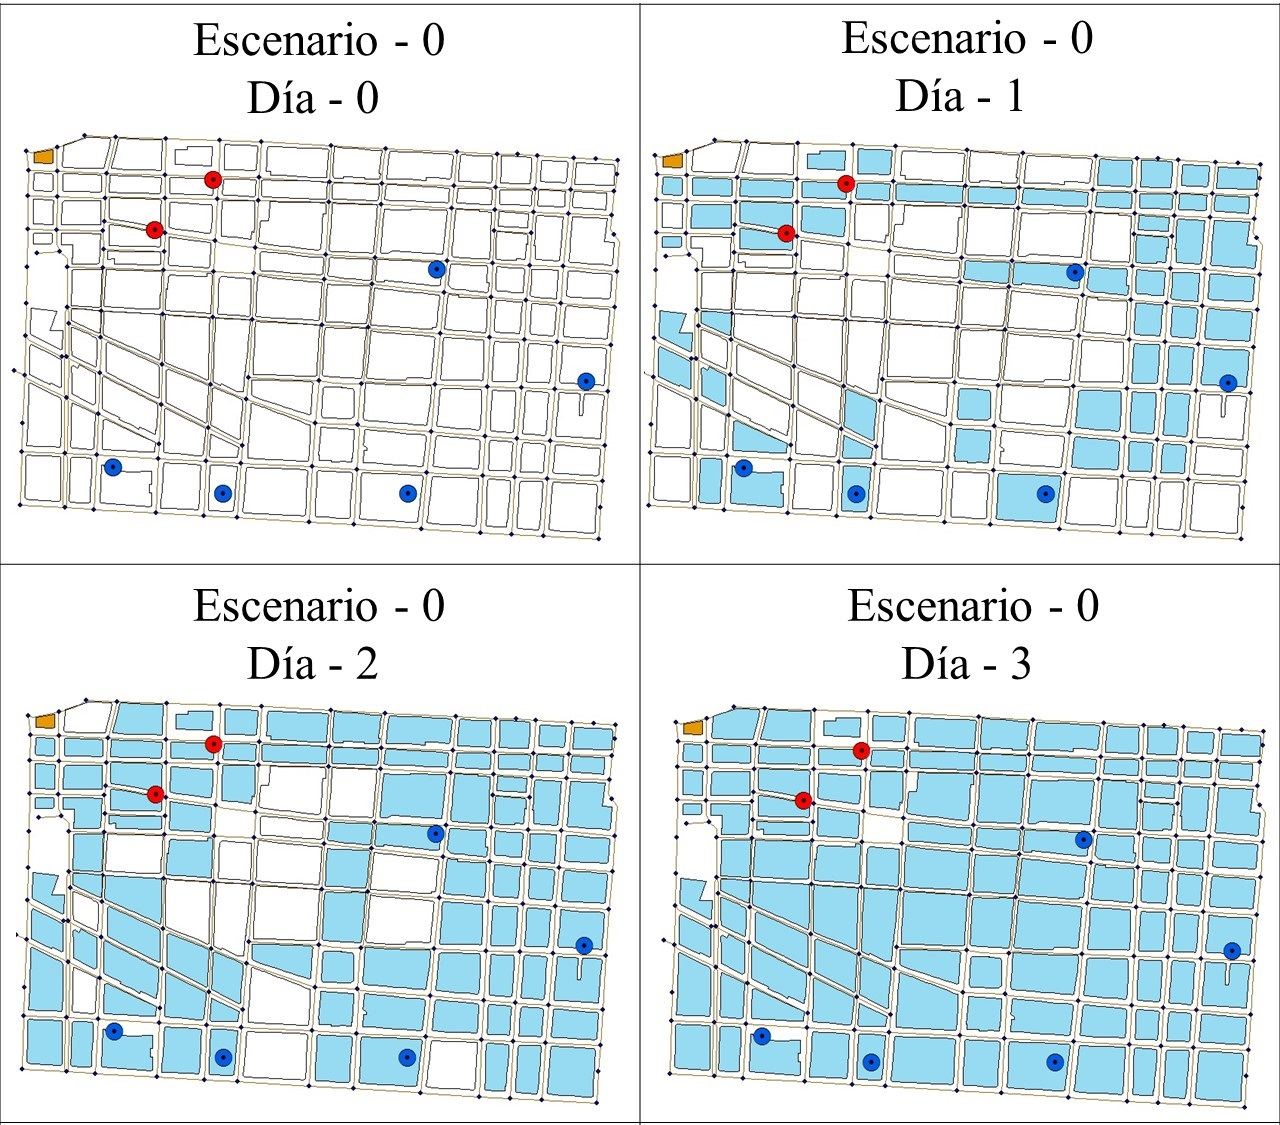
\includegraphics[scale=0.3]{Figuras/visu1.jpg}
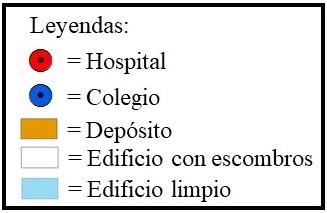
\includegraphics[scale=0.4]{Figuras/simb2.jpg} 
\caption{Visualización de edificios limpios  (Escenario 0), Fuente: Elaboración propia}
\label{fig:esc0-visu}
\end{figure}

%%%%%%%%%%%%%%%%%%%%%%%%%%%%%%%%%%%%%%%%%%%%%%%%%%%%%%%%%%%%%%%%%%%%%%%%%%%%%

En resumen, del escenario 0 se puede concluir que el modelo sí realiza una priorización exitosa al considerar los ponderadores de tipo de edificio y día, puesto que en la Figura \ref{fig:esc0-graf} se muestra cómo se agrupa la mayor cantidad de edificios en los primeros días y en la Figura \ref{fig:esc0-visu} que los primeros en limpiarse son los de mayor prioridad y luego los que presentan mayores escombros. Asimismo, mediante los indicadores se vuelve a verificar el coeficiente de prioridad limpiando los hospitales y colegios en el primer día de trabajo.

\section{Análisis de la metodología sin factor de preferencia (Escenario 1)}

En este análisis se detalla cómo se comporta el modelo sin los factores de preferencia. En la Tabla \ref{tab:comp01} se muestran los resultados.


%%%%%%%%%%%%%%%%%%%%%%%%%%%%%%%%%%%%%%%%%%%%%%%%%%%%%%%%%%%%%%%%%%%%%%%%%%%

\begin{table}[h!]
\resizebox{15cm}{!} {
\begin{tabular}{c|c|c|c|c|c|c|c|c|c}
\hline
\multirow{3}{*}{Escenario} & Función                   & Tiempo & GAP                   & Edificios                & Cant. prom. de                 & No. prom. de días & \multicolumn{3}{c|}{Cant. de días promedio de limpieza}                          \\ \cline{8-10} 
                           & \multirow{2}{*}{objetivo} & CPU    & \multirow{2}{*}{(\%)} & \multirow{2}{*}{Limpios} & escombros recolectados         & para limpiar      & \multirow{2}{*}{Hospitales} & \multirow{2}{*}{Colegios} & \multirow{2}{*}{Otros} \\
                           &                           & (seg)  &                       &                          & por día m\textasciicircum{}(3) & un edificio       &                             &                           &                        \\ \hline
0                          & 103                       & 18000  & 1.33                  & 108                      & 1,254.97                       & 2.26              & 1                           & 1                         & 1.67                   \\ 
1                          & 117                       & 40     & 0.00                  & 108                      & 752.25                         & 2.26              & 2.53                        & 3                         & 2.5                    \\ \hline
\end{tabular}
}
\caption{Detalle comparación Escenarios 0 y 1, Fuente: Elaboración propia. }
\label{tab:comp01}
\end{table}

%%%%%%%%%%%%%%%%%%%%%%%%%%%%%%%%%%%%%%%%%%%%%%%%%%
El modelo matemático se ejecutó por 40 segundos, obteniendo un GAP del $0.00\%$ debido que al quitar el factor de preferencia se simplifica ejecutar el modelamiento. En esta instancia, al igual que en la anterior se limpiaron 108 edificios y la cantidad de escombros recolectada es 3.761,23 $m^{3}$.

En la Figura \ref{fig:esc01graf} se presenta el gráfico de la cantidad de edificios limpiados por día, donde se aprecia que, al eliminar el factor de preferencia se realiza una limpieza constante, distinto lo que hace el escenario 0. Además se puede confirmar la limpieza contante a causa de la utilización de los 5 días del horizonte de planificación. Asimismo mediante los indicadores, se verifica una menor cantidad de escombros recolectados por día, destacando un rendimiento uniforme durante el horizonte de planificación.


\begin{figure}[h!]
\centering
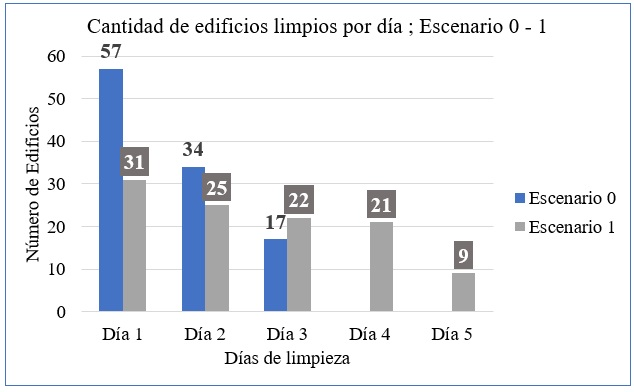
\includegraphics[scale=0.8]{Figuras/INDIC2.jpg} 
\caption{Detalle de edificios limpios (Escenarios 0 y 1), Fuente: Elaboración propia}
\label{fig:esc01graf}
\end{figure}



%%%%%%%%%%%%%%%%%%%%%%%%%%%%%%%%%%%%%%%%%%%%%%%%%%
La distribución espacial de limpieza de los edificios se ve representada en la Figura \ref{fig:esc01-visu}, donde se visualiza cómo se van limpiando los edificios a medida que pasan los días. Aquí se observa la comparación de los primeros 3 días del horizonte de planificación demostrando la limpieza constante versus el comportamiento de la limpieza con el factor de preferencía de limpieza hacia los primeros días de trabajo.


\begin{figure}[h!]
\centering
\includegraphics[scale=0.3]{Figuras/visu2.jpg} 
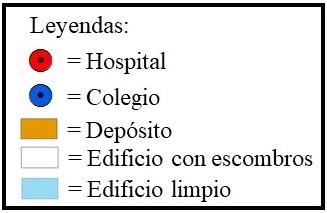
\includegraphics[scale=0.4]{Figuras/simb2.jpg}
\caption{Visualización de edificios limpios  (Escenarios 0 y 1), Fuente: Elaboración propia}
\label{fig:esc01-visu}
\end{figure}


%%%%%%%%%%%%%%%%%%%%%%%%%%%%%%%%%%%%%


En resumen, del escenario 1 se puede concluir que el modelo realiza un rendimiento constante en cuanto a limpieza puesto que en la Figura \ref{fig:esc01graf} se muestra una comparación del horizonte de planificación, representando un número de limpieza constante en el escenario 1 y la priorización de la limpieza hacia los primeros días en el escenario 0. Además en la Figura \ref{fig:esc01-visu} se realiza la comparación respectiva de los primeros 3 días del horizonte de planificación, donde representa la falencía en la limpieza del escenario 1. Asimismo, mediante los indicadores se puede comprobar que la variación afecta directamente a la prioridad de limpiar Hospitales y colegios, aumentando considerablemente el tiempo en habilitar los edificios mencionados.

%%%%%%%%%%%%%%%%%%%%%%%%%%%%%%%%%%%%%%%%%%

%Presentarla igual que en el primer escenario, sin números, mostrando solo los indicadores que te mostré. Luego explicar y mostrar el gráfico de la comparación de escenarios 0 y 1. Terminas con la figura de los 4 mapas, explicando de la misma manera que lo hcie en 1.

%%%%%%%%%%%%%%%%%%%%%%%%%%%%%%%%%%%%%%%%%%%%%%%%%%%%%%%%%%%%%%%%%%%%%%%%%%%%%

\section{Análisis de variación en el recurso vehicular (Escenarios 2 y 3)}

En este análisis se detalla cómo se comporta el modelo variando la cantidad de vehículos operativos. En la Tabla \ref{tab:comp02} se muestran los resultados.
\begin{table}[h!]
\resizebox{15cm}{!} {
\begin{tabular}{c|c|c|c|c|c|c|c|c|c}
\hline
\multirow{3}{*}{Escenario} & Función                   & Tiempo & GAP                   & Edificios                & Cant. prom. de                 & No. prom. de días & \multicolumn{3}{c|}{Cant. de días promedio de limpieza}                          \\ \cline{8-10} 
                           & \multirow{2}{*}{objetivo} & CPU    & \multirow{2}{*}{(\%)} & \multirow{2}{*}{Limpios} & escombros recolectados         & para limpiar      & \multirow{2}{*}{Hospitales} & \multirow{2}{*}{Colegios} & \multirow{2}{*}{Otros} \\
                           &                           & (seg)  &                       &                          & por día m\textasciicircum{}(3) & un edificio       &                             &                           &                        \\ \hline
0                          & 103                       & 18000  & 1.33                  & 108                      & 1,254.97                       & 2.26              & 1                           & 1                         & 1.67                   \\ 
2                          & 78                        & 18000  & 7.21                  & 99                       & 658.34                         & 1.99              &  1                       & 1.4                          & 2.57                   \\
3                          & 109                       & 18000  & 1.48                  & 107                      & 1,863.41                       & 2.24              & 1                           & 1                         & 1.32                   \\ \hline
\end{tabular}
}
\caption{Detalle comparación Escenarios 0, 2 y 3, Fuente: Elaboración propia. }
\label{tab:comp02}
\end{table}

%%%%%%%%%%%%%%%%%%%%%%%%%%%%%%%%%%%%%%%%

Ambos modelos matemáticos de los escenarios 2 y 3 se ejecutaron por 5 horas, obteniendo un GAP de $7.21\%$ y $1.48\%$ respectivamente. En estas instancias, se limpiaron 99 y 107 edificios y  la cantidad de escombros recolectada es de  3.291,71 $m^{3}$  y  3.726,81 $m^{3}$ respectivamente.
En la Figura \ref{fig:esc023graf} se presenta el gráfico de la cantidad de edificios limpiados por día, donde se aprecia que, existe dificultad de trabajar con 5 camiones en el escenario 2 y la facilidad del escenario 3 en cumplir el objetivo de realizar la limpieza global en solo 2 días, debido que cuenta con 15 camiones operativos. Además se puede destacar que los modelos propuestos utilizaron de excelente manera los recursos proporcionados, limpiando los edificios de mayor prioridad en el primer día del horizonte de  planificación.

%%%%%%%%%%%%%%%%%%%%%%%%%%%%%%%%%%%%%%%%%%%%


\begin{figure}[h!]
\centering
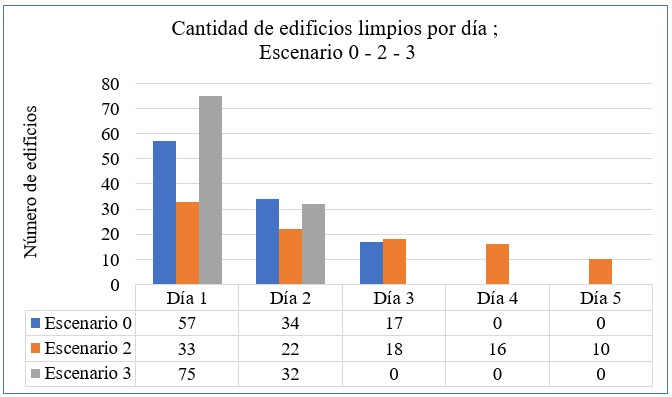
\includegraphics[scale=0.8]{Figuras/INDIC3.jpg} 
\caption{Detalle de edificios limpios (Escenarios 0, 2 y 3), Fuente: Elaboración propia}
\label{fig:esc023graf}
\end{figure}

%%%%%%%%%%%%%%%%%%%%%%%%%%%%%%%%%


La distribución espacial de limpieza de los edificios se ve representada en la Figura \ref{fig:esc023-visu}, donde se visualiza cómo se van limpiando los edificios a medida que pasan los 2 primeros días de trabajo. Aquí se observa la comparación de los edificios completamente limpios durante el horizonte de planificación de los 3 escenarios, representando la diferencia en cuanto a proporción de recursos utilizados, presentando un deficit de cantidad de edificios limpios en el escenario 2 y una ventaja en cuanto a la limpieza de edificios en el escenario 3 ambos siendo comparados con el escenario 0.

\begin{figure}[h!]
\centering
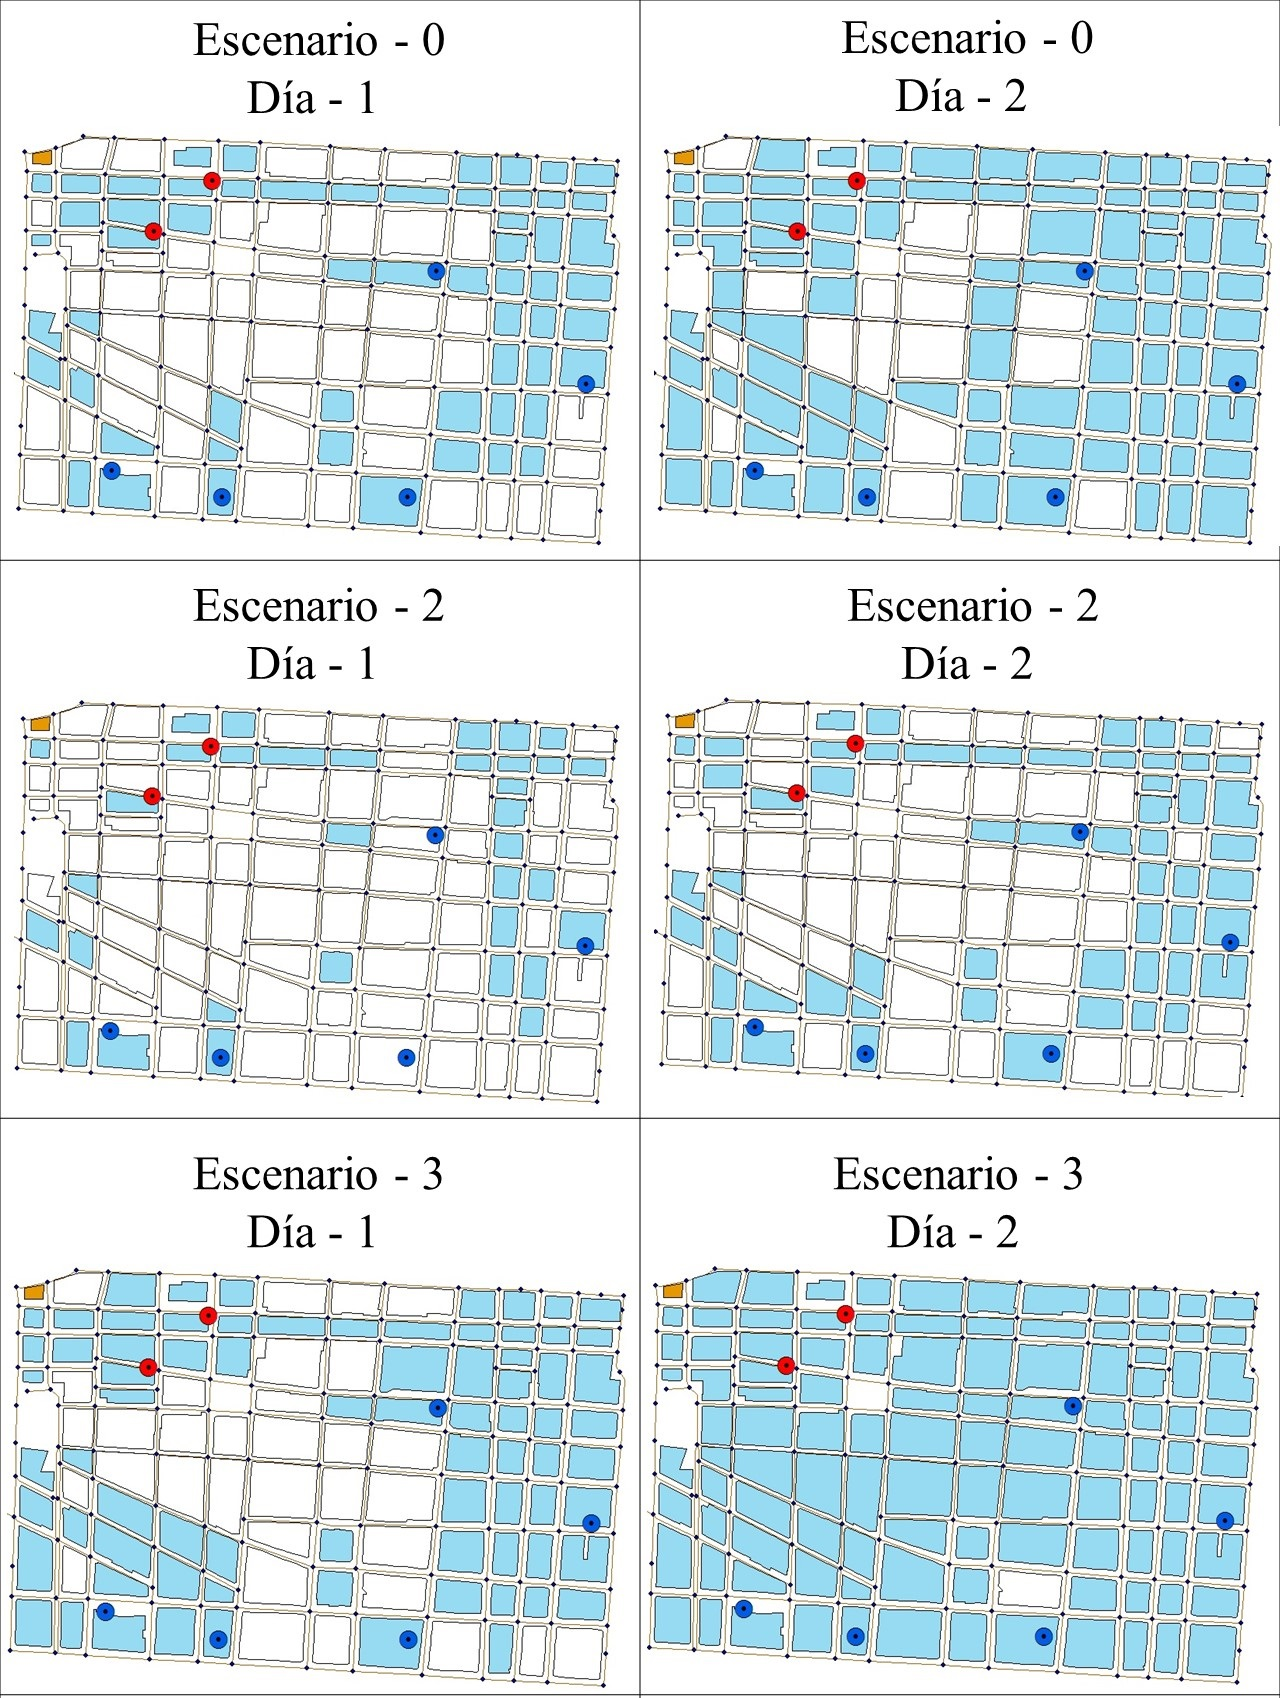
\includegraphics[scale=0.3]{Figuras/visu3.jpg} 
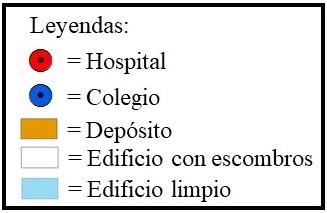
\includegraphics[scale=0.4]{Figuras/simb2.jpg} 
\caption{Visualización de edificios limpios  (Escenarios 0, 2 y 3), Fuente: Elaboración propia}
\label{fig:esc023-visu}
\end{figure}
	
%%%%%%%%%%%%%%%%%%%%%%%%%%%%%%%%%%%%%%

En resumen, de los escenarios 2 y 3 se puede concluir que los modelos si realizan una priorización exitosa de los ponderadores de tipo de edificio y día, puesto que en la Figura \ref{fig:esc023graf} se muestra una comparación del horizonte de planificación, representando la priorización de limpieza en el primer día del horizonte de planificación. Además en la Figura \ref{fig:esc023-visu} se realiza la comparación respectiva de los primeros 2 días del horizonte de planificación, donde representa la importancia de contar con los recursos suficientes para realizar los trabajos respectivos de limpieza. Asimismo, mediante los indicadores se puede comprobar que la variación no afecta la priorización de limpieza de los edificios tales como Hospitales y colegios.

\section{Análisis de variación en la cantidad de escombros (Escenarios 4, 5 y 6)}

En este análisis se detalla cómo se comporta el modelo aumentando la cantidad de volumen de escombros de cada edificio. En la Tabla \ref{tab:comp03} se muestran los resultados.

\begin{table}[h!]
\resizebox{15cm}{!} {
\begin{tabular}{c|c|c|c|c|c|c|c|c|c}
\hline
\multirow{3}{*}{Escenario} & Función                   & Tiempo & GAP                   & Edificios                & Cant. prom. de                 & No. prom. de días & \multicolumn{3}{c|}{Cant. de días promedio de limpieza}                          \\ \cline{8-10} 
                           & \multirow{2}{*}{objetivo} & CPU    & \multirow{2}{*}{(\%)} & \multirow{2}{*}{Limpios} & escombros recolectados         & para limpiar      & \multirow{2}{*}{Hospitales} & \multirow{2}{*}{Colegios} & \multirow{2}{*}{Otros} \\
                           &                           & (seg)  &                       &                          & por día m\textasciicircum{}(3) & un edificio       &                             &                           &                        \\ \hline
0                          & 103                       & 18000  & 1.33                  & 108                      & 1,254.97                       & 2.26              & 1                           & 1                         & 1.67                   \\ 
4                          & 99                        & 18.000 & 3.83                  & 104                      & 1.204,30                       & 2.29              & 1                           & 1.2                       & 1.69                   \\ 
5                          & 98                        & 18.000 & 2.65                  & 106                      & 738.44                         & 2.59              & 1                           & 1.2                       & 1.83                   \\ 
6                          & 96                        & 18.000 & 2.34                  & 106                      & 926.04                         & 2.75              & 1                           & 1.2                       & 1.92                   \\ \hline
\end{tabular}
}
\caption{Detalle comparación Escenarios 0, 4, 5 y 6 Fuente: Elaboración propia. }
\label{tab:comp03}
\end{table}

%%%%%%%%%%%%%%%%%%%%%%%%%%%%%%%%%%%%%%%%%%%%

Los 3 modelos matemáticos de los escenarios 4, 5 y 6 se ejecutaron por 5 horas, obteniendo un GAP de $3.83\%$, $2.65\%$ y $2.34\%$ respectivamente. En estas instancias, se limpiaron 104 edificios en el escenario 4 y 106 edificios en los escenarios 5 y 6. La cantidad de escombros recolectada es de  3,612.89 $m^{3}$, 3.692,21 $m^{3}$  y  3.704,18 $m^{3}$ respectivamente.
En la Figura \ref{fig:esc0456graf} se presenta el gráfico de la cantidad de edificios limpiados por día, donde se aprecia que, al aumentar la cantidad de volumen de escombros por edificio, se presenta una menor cantidad de edificios limpios en comparación al escenario 0 y a la vez se puede visualizar la priorización correcta, de limpieza de los edificios hacia los primeros días del horizonte de planificación siendo comprobado por la cantidad de edificios completamente limpios en los primeros 3 días de trabajo.


%%%%%%%%%%%%%%%%%%%%%%%%%%%%%%%%%%%%%%%%%%%%%%%%%%%%%%%%%%%%%%%%%%%%%%%%%%%
\begin{figure}[h!]
\centering
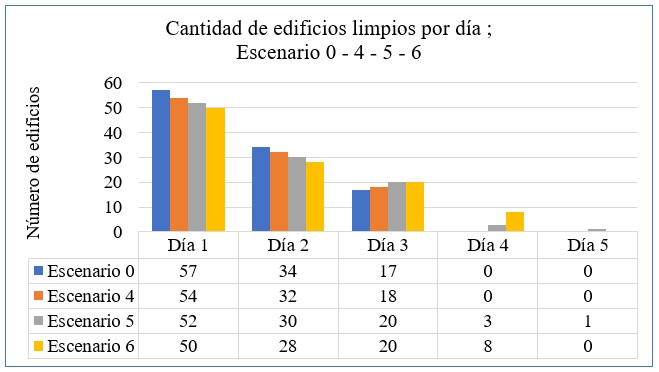
\includegraphics[scale=0.8]{Figuras/INDIC4.jpg} 
\caption{Detalle de edificios limpios (Escenarios 0, 4, 5 y 6), Fuente: Elaboración propia}
\label{fig:esc0456graf}
\end{figure}


%%%%%%%%%%%%%%%%%%%%%%%%%%%%

La distribución espacial de limpieza de los edificios se ve representada en la Figura \ref{fig:esc0456-visu}, donde se visualiza cómo se van limpiando los edificios durante el primer y tercer día de trabajo. Aquí se observa la comparación de los edificios completamente limpios durante el horizonte planificación de los 4 escenarios, representando como aumenta la dificultad al incrementar el volumen de escombros por edificio, presentando una visualización del decrecimiento de edificios completamente limpio en cada escenario respectivo.

\begin{figure}[h!]
\centering
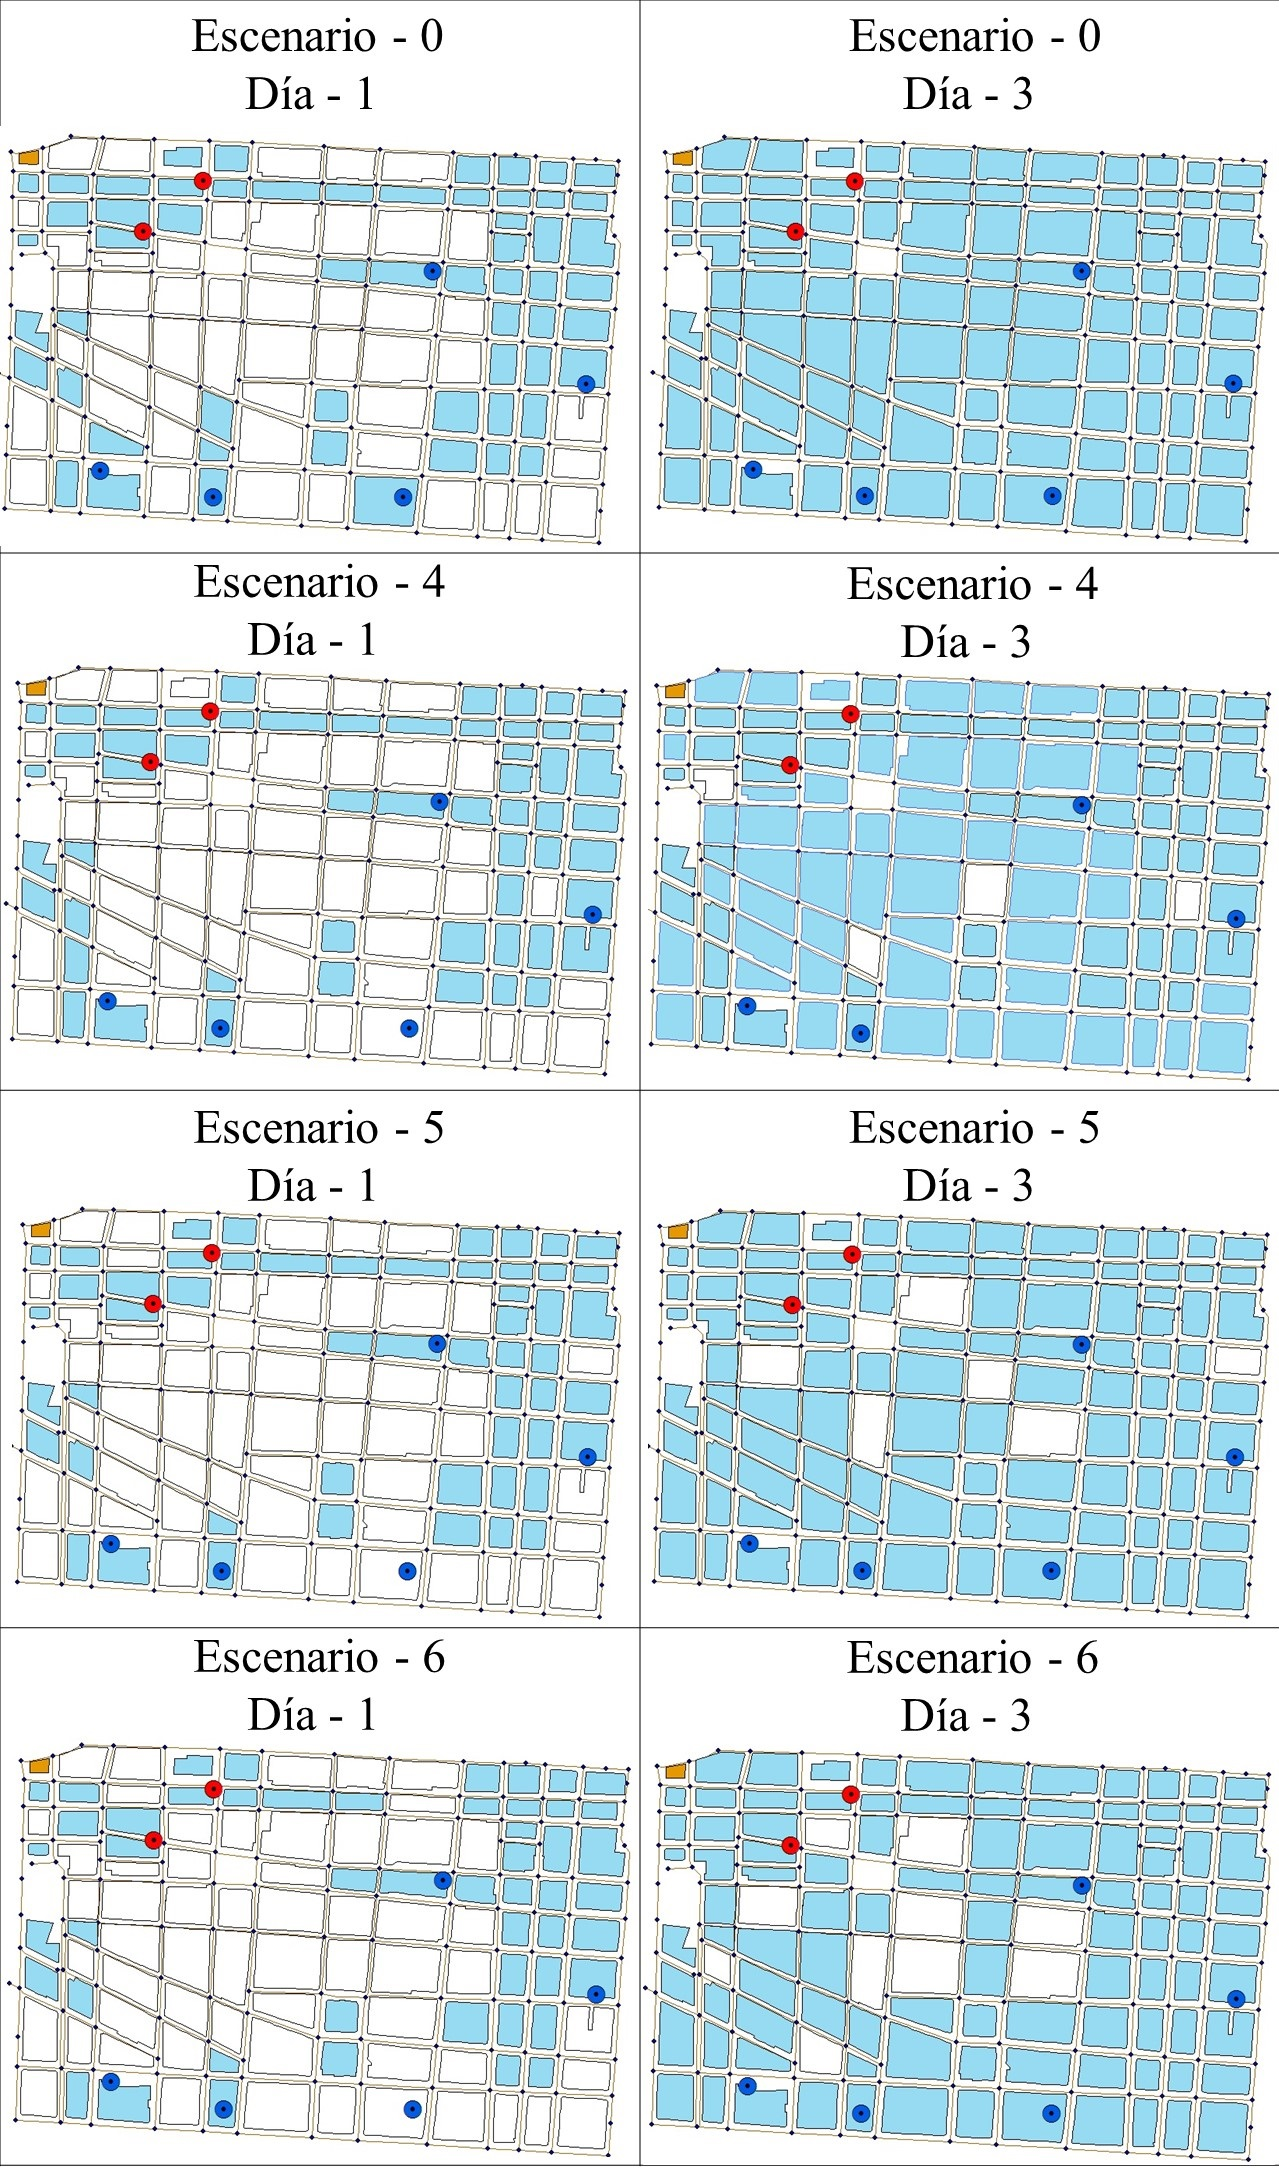
\includegraphics[scale=0.25]{Figuras/visu4.jpg}
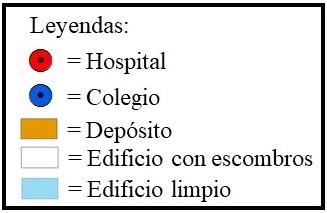
\includegraphics[scale=0.4]{Figuras/simb2.jpg}  
\caption{Visualización de edificios limpios  (Escenarios 0, 2 y 3), Fuente: Elaboración propia}
\label{fig:esc0456-visu}
\end{figure}

%%%%%%%%%%%%%%%%%%%%%%%%%%%%%%

\pagebreak

En resumen, de los escenario 4, 5 y 6 se puede concluir que los  modelos si realizan una priorización exitosa de los ponderadores de tipo de edificio y día, puesto que en la Figura \ref{fig:esc0456graf} se muestra una comparación del horizonte de planificación, representando la priorización de limpieza en el primer día del horizonte de planificación. Además en la Figura \ref{fig:esc0456-visu} se realiza la comparación respectiva de los primer y tercer día del horizonte de planificación, donde representa dificultad de realizar la limpieza al aumentar el volumen de escombros, disminuyendo considerablemente el numero de edificios completamente limpio. Además mediante los indicadores, se verifica que el modelo responde correctamente a la priorización de limpieza de los edificios en el primer día de trabajo.

%%%%%%%%%%%%%%%%%%%%%%%%%%%%%

%Una vez que terminas de rellenar todo esto, es lo mismo en el paper y en la PPT.

%%%%%%%%%%%%%%%%%%%%%%%%%%%%%%%%%%%%%%%%%%%%%%%%%%%%%%%%%%%%%%%%%%%%%%%%%%%%%

\section{CONCLUSIÓN Y TRABAJOS FUTUROS}

En esta investigación se desarrolló una metodología que permite tomar decisiones tácticas y operativas, puesto que es capaz de planificar la asignación de recursos claves posterior de ocurrir un desastre natural y dentro de un horizonte de planificación. Además, el modelo realiza consideraciones de elementos como capacidad de carga de camión, volumen de escombros por edificio, distribución espacial de los edificios con prioridad de estar completamente limpios.  Asimismo, considera el objetivo de realizar la preferencia de limpieza de los edificios hacia los primeros días del horizonte de planificación, además de priorizar los edificios que más ayudan a la población en el caso de un desastre, los cuales son los hospitales y centros de educación.

Posteriormente, se comprueba el modelo propuesto en un escenario base, en una instancia menor a la totalidad de la ciudad propuesta en el caso de estudio, con características experimentales tales como número de camiones, número de vueltas y número de días. Consecutivamente, se realiza diversos análisis de variación del escenario base, presentando variaciones en quitar el factor de preferencia, variar la cantidad de camiones operativos y aumentar la cantidad de volumen de escombros. 

Los resultados de cada escenario propuesto fueron comparados con el escenario base, para verificar cómo se comporta el modelo y comprobar que la cantidad de edificios completamente limpios no afecte en el objetivo general, limpiando la mayor cantidad de edificios hacia los primeros días del horizonte de planificación. Los resultados en general se consideran favorables para la modelación, a causa de que la mayoría de los modelos limpia favorablemente los edificios con priorización, es decir hospitales y colegios.

Si bien el problema se puede resolver computacionalmente en un tiempo razonable, cuando se tiene una instancia mayor presenta prolongados tiempos de computo, por lo cual en un trabajo a futuro se podría presentar una heurística que permita desarrollar resultados en menores tiempos de modelación. A la vez se debería considerar incluir el rendimiento de bulldozer para obtener tiempos en la operación completa y finalmente completando el equipo de limpieza con la inclusión de una retroexcavadora para remover los materiales distintos de madera y ladrillos. También para obtener un mejor provecho de la remoción de escombros en general, se podría considerar algún tipo de zonas de almacenamiento temporal, ya sean plazas y/o terrenos sin habitantes ni construcciones, para poder recolectar de manera provisional escombros, cuyo beneficio se reflejaría en el tiempo de transito de los camiones recolectores. En esté caso no se menciona aspectos de reciclajes, por lo cual se consideraría una desventaja al largo plazo, es importante incluir los equipos que podrían realizar reciclaje para reutilizar los materiales de construcción.  Asimismo, se deberían considerar múltiples depósitos para gestionar una mayor capacidad de escombros, en el mejor caso agregar un parámetro de generación de depósitos de ser necesario. Finalmente, se debería incorporar el traslado de escombros entre nodos para agilizar la habilitación de los edificios con mayor priorización tales como hospitales, colegios y albergues.

\pagebreak

\section{REFERENCIAS BIBLIOGRÁFICAS}

\bibliographystyle{apalike}
\bibliography{references}

\pagebreak

\section{ANEXOS}

\subsection{Detalle de edificios} \label{anexo1}

\begin{table}[htb!]
	\centering
	\begin{tabular}{|c|c|c|}
\hline 
Código & Nombre                         & Descripción \\  \hline
H1     & PRAIS SS IQUIQUE               & Hospital    \\  
H2     & H. DR ERNESTO TORRES GALDAMEZ  & Hospital    \\  
H3     & CESFAM CIRUJANO AGUIRRE        & Hospital    \\  
H4     & CESFAM CIRUJANO VIDELA         & Hospital    \\  
H5     & CESFAM SUR DE IQUIQUE          & Hospital    \\  
H6     & SAPU CIRUJANO AGUIRRE          & Hospital    \\  
H7     & SAPU CIRUJANO VIDELA           & Hospital    \\  
H8     & SAPU SUR DE IQUIQUE            & Hospital    \\  
H9     & POLI TRABAJADOR ACHS IQUIQUE   & Hospital    \\  
H10    & C.A. DE INSTITUTO DE SEGURIDAD & Hospital    \\  
H11    & POLI.  CARABINEROS DE IQUIQUE  & Hospital    \\  
H12    & CLINICA DENTAL MOVIL SIMPLE    & Hospital    \\  
H13    & C. S. DE MUTUAL CCHC IQUIQUE   & Hospital    \\  
H14    & CLINICA TARAPACA               & Hospital    \\  
H15    & CLINICA IQUIQUE                & Hospital    \\  
H16    & CENTRO CLINICO MILITAR IQUIQUE & Hospital    \\  
C1     & L. ALMIRANTE CARLOS CONDELL      & Colegio     \\  
C2     & COL. LIRIMA                      & Colegio     \\  
C3     & ESC. DE LENGUAJE NUEVO INTI      & Colegio     \\  
C4     & COL. SAMCA ARUMANTI              & Colegio     \\  
C5     & COL. ANTAMARA                    & Colegio     \\  
C6     & COL. LATINOAMERICANO LAS PARINAS & Colegio     \\  
C7     & COL. HISPANO BRITANICO IQUIQUE   & Colegio     \\  
C8     & COL. MAHATMA GANDHI              & Colegio     \\  
C9     & L. COL. DEPORTIVO                & Colegio     \\  
C10    & EAGLES COLLEGE                   & Colegio     \\  
C11    & COL. SUEÑO DEL MAÑANA            & Colegio     \\  
C12    & COL. NIMARA                      & Colegio     \\  
C13    & ESC. BASICA CHIPANA              & Colegio     \\  
C14    & COL. DE LA COSTA                 & Colegio     \\  
C15    & COL. GOLDEN NORTH                & Colegio     \\  
C16    & ACADEMIA NERUDIANA               & Colegio     \\  
C17    & COL. HUMBERSTONE                 & Colegio     \\  
C18    & COL. MARIA REINA                 & Colegio     \\  
C19    & ESC. PR.L CASTRO RAMOS           & Colegio     \\  
C20    & COL. REPUBLICA DE ITALIA         & Colegio     \\  
C21    & L. LUIS CRUZ MARTINEZ            & Colegio     \\  
C22    & COL. ESPANA                      & Colegio     \\  
C23    & COL. LITTLE STARS                & Colegio     \\  
C24    & ESC. THILDA PORTILLO OLIVARES    & Colegio     \\  
C25    & COL. NIMARA                      & Colegio     \\  \hline
\end{tabular}
\end{table}

\begin{table}[h!]
	\centering
	\begin{tabular}{|c|c|c|}
\hline
C26    & COL. REPUBLICA DE CROACIA        & Colegio     \\  
C27    & ESC. GABRIELA MISTRAL            & Colegio     \\  
C28    & L. JOSE GUTIERREZ DE LA FUENTE   & Colegio     \\  
C29    & COL. ADVENTISTA DE IQUIQUE       & Colegio     \\  
C30    & ESC. DOMINGO SANTA MARIA         & Colegio     \\ 
C31    & L. PARTICULAR MIXTO ESCASCE      & Colegio     \\  
C32    & L. PR. ANIBAL PINTO GARMENDIA    & Colegio     \\  
C33    & COL. IQUIQUE YOUNG SCHOOL        & Colegio     \\  
C34    & COL. SALESIANO DE IQUIQUE        & Colegio     \\  
C35    & COL. NORTH COLLEGE               & Colegio     \\  
C36    & COL. INGLES                      & Colegio     \\  
C37    & L. MARIA AUXILIADORA             & Colegio     \\  
C38    & COL. HISPANO ITALIANO            & Colegio     \\  
C39    & L. SUPERIOR GABRIELA MISTRAL     & Colegio     \\  
C40    & ESC. P.JARAQUEMADA ALQUIZAR      & Colegio     \\  
C41    & ESC. ARTISTICA VIOLETA PARRA     & Colegio     \\  
C42    & COL. ACADEMIA TARAPACA ORELLA    & Colegio     \\  
C43    & COL. HUANTAJAYA                  & Colegio     \\  
C44    & ESC. PLACIDO VILLAROEL           & Colegio     \\  
C45    & L. LIBERTADOR BERNARDO OHIGGINS  & Colegio     \\  
C46    & I.COMEX BALDOMERO WOLNITZKY      & Colegio     \\  
C47    & L.COMEX MIRADA DE COLORES        & Colegio     \\  
C48    & COL. BULNES                      & Colegio     \\  
C49    & COL. NUSTA KORI                  & Colegio     \\  
C50    & ESC. BASICA CORONA SCHOOL        & Colegio     \\  
C51    & COL. ACADEMIA TARAPACA ORELLA    & Colegio     \\  
C52    & COL. UNIVERSITARIO UNAP          & Colegio     \\  
C53    & L. ELENA DUVAUCHELLE CABEZON     & Colegio     \\  
C54    & ESC. JAVIERA CARRERA VERDUGO     & Colegio     \\  
C55    & COL. IRQUILLARIY                 & Colegio     \\  
C56    & ESC. BASICA FRANCISCO FORGIONE   & Colegio     \\  
C57    & L. ATENEA                        & Colegio     \\  
C58    & COL. LITTLE COLLEGE              & Colegio     \\  
C59    & ESC. EDUARDO LLANOS              & Colegio     \\  
C60    & ESC. CENTENARIO                  & Colegio     \\  
C61    & COL. SAINT MARGARET ROSE GARDEN  & Colegio     \\  
C62    & SEMILLA DE CRISTO L. ARTURO      & Colegio     \\  
C63    & LIC. COMEX Y TECNICO ARTURO PRAT & Colegio     \\  
C64    & COL. DIOCESANO OBISPO LABBE      & Colegio     \\  
C65    & ESC. ALMIRANTE PATRICIO LYNCH    & Colegio     \\  \hline
\end{tabular}
	\caption {Detalle de edificios relevantes en la zona ; Fuente: \citep{CENSO2017}}
	\label{tab3}
\end{table}

%%%%%%%%%%%%%%%%%%%%%%%%%%%%%%%%%%%%%%%%%%%%%%%%%%%%%%%%%%%%%

%REF2 = pon la misma referencia que en la red vial.

%%%%%%%%%%%%%%%%%%%%%%%%%%%%%%%%%%%%%%%%%%%%%%%%%%%%%%%%%%%%%%

\end{document}